\chapter{OSPF: Part 3}\label{ospf-part-3}

\section{Loopback Interfaces}\label{loopback-interfaces}

\begin{itemize}
\tightlist
\item
  A LOOPBACK INTERFACE is a virtual INTERFACE in the ROUTER
\item
  It is ALWAYS UP/UP - unless you manually shut it down
\item
  It is NOT dependent on a PHYSICAL INTERFACE
\item
  So, it provides a consistent IP ADDRESS that can be used to REACH /
  IDENTIFY the ROUTER
\end{itemize}

\begin{figure}
\centering
\pandocbounded{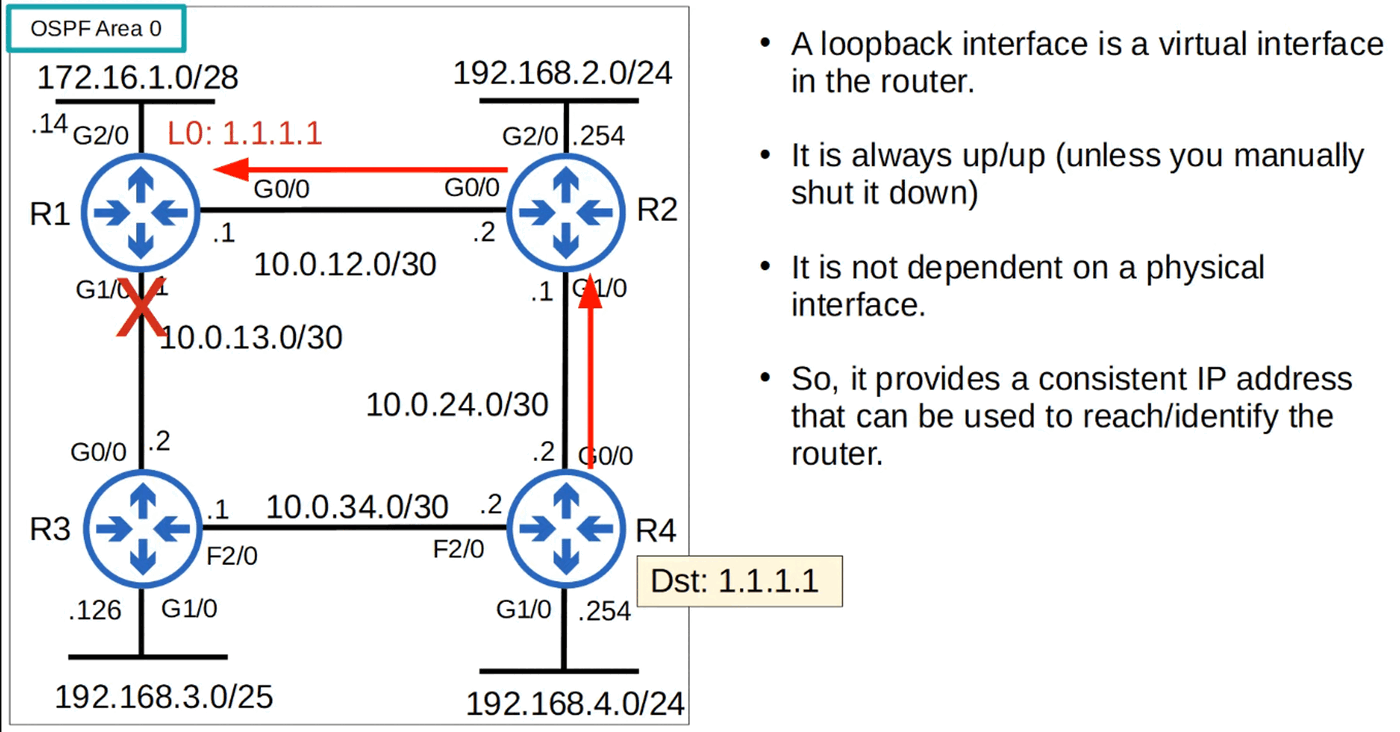
\includegraphics[keepaspectratio,alt={image}]{images/29-ospf-part3/img-001.png}}
\end{figure}

\section{OSPF Network Types}\label{ospf-network-types}

\begin{itemize}
\item
  The OSPF ``NETWORK TYPE'' refers to the TYPES of connection between
  OSPF neighbors (Ethernet, etc.)
\item
  There are THREE MAIN OSPF NETWORK TYPES:
\item
  BROADCAST :

  \begin{itemize}
  \tightlist
  \item
    Enabled by DEFAULT on \textbf{ETHERNET} and \textbf{FDDI} (Fiber
    Distributed Data Interfaces) INTERFACES
  \end{itemize}
\item
  POINT TO POINT :

  \begin{itemize}
  \tightlist
  \item
    Enabled by DEFAULT on \textbf{PPP} (Point-to-Point) and
    \textbf{HDLC} (High-Level Data Link Control) INTERFACES
  \end{itemize}
\item
  NON-BROADCAST :

  \begin{itemize}
  \tightlist
  \item
    Enabled by DEFAULT on \textbf{FRAME RELAY} and \textbf{X.25}
    INTERFACES
  \end{itemize}
\end{itemize}

\begin{tipbox}

CCNA focuses on BROADCAST and POINT-TO-POINT types

\end{tipbox}

\section{OSPF Broadcast Network Type}\label{ospf-broadcast-network-type}

\begin{figure}
\centering
\pandocbounded{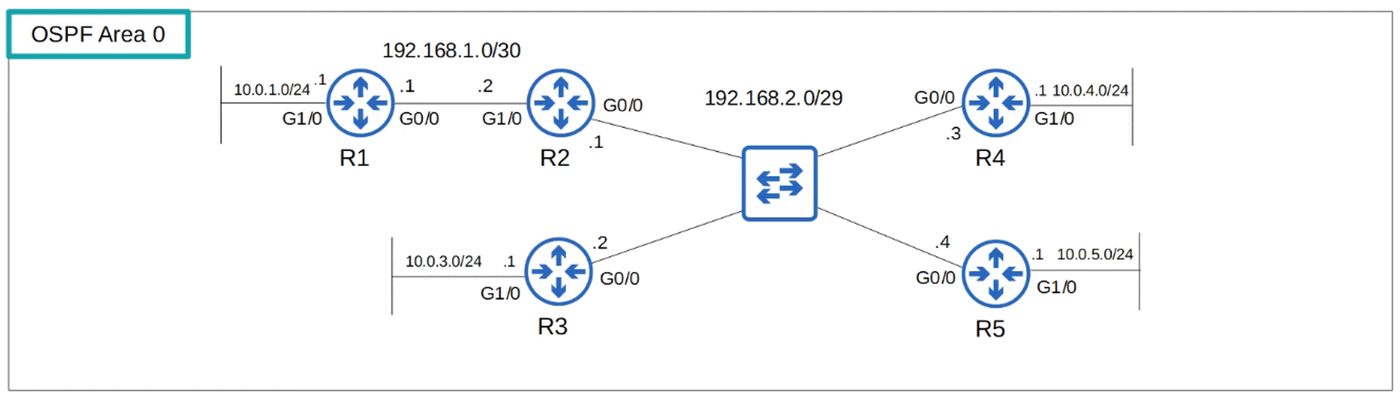
\includegraphics[keepaspectratio,alt={image}]{images/29-ospf-part3/img-002.png}}
\end{figure}

\begin{itemize}
\tightlist
\item
  Enabled on ETHERNET and FDDI interfaces by DEFAULT
\item
  ROUTERS \emph{dynamically discover} neighbors by SENDING / LISTENING
  for OSPF ``Hello'' messages using the multicast address 224.0.0.5
\item
  A \textbf{DR (DESIGNATED ROUTER)} and \textbf{BDR (BACKUP DESIGNATION
  ROUTER)} must be elected on each subnet (only DR if there are no OSPF
  neighbors, ie: R1's G1/0 INTERFACE)
\item
  ROUTERS which aren't the DR or BDR become a \textbf{DROther}
\end{itemize}

\begin{figure}
\centering
\pandocbounded{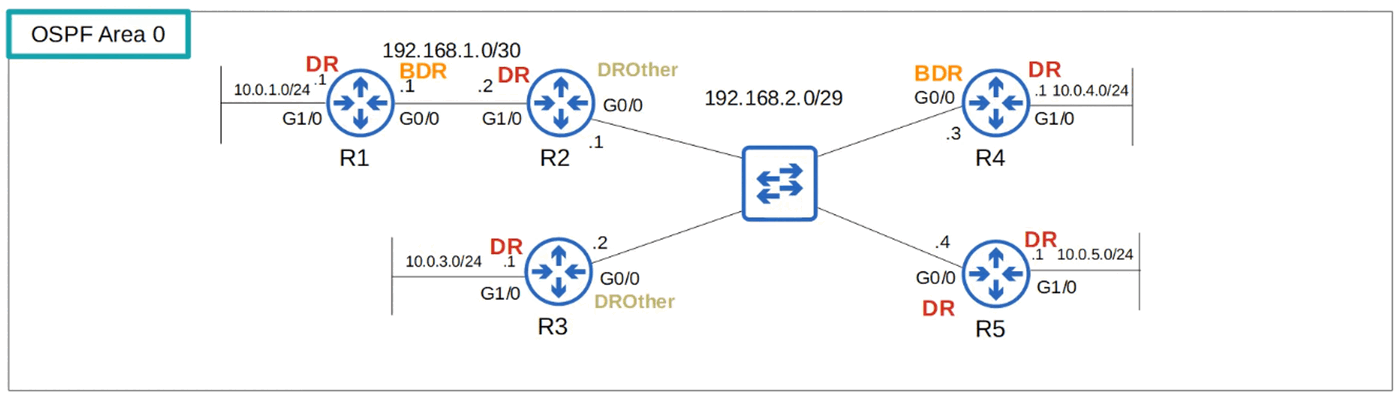
\includegraphics[keepaspectratio,alt={image}]{images/29-ospf-part3/img-003.png}}
\end{figure}

The DR / BDR election order of priority:

\begin{enumerate}
\def\labelenumi{\arabic{enumi})}
\item
  Highest OSPF INTERFACE PRIORITY
\item
  Highest OSPF ROUTER ID
\end{enumerate}

``First Place'' becomes the DR for the SUBNET

``Second Place'' because the BDR

\begin{tipbox}

DEFAULT OSPF INTERFACE PRIORITY is ``1'' on ALL INTERFACES!

\end{tipbox}

The command to change the OSPF PRIORITY of an INTERFACE is :

\begin{tipbox}

R2(config-if)\# ip ospf priority \textless priority number\textgreater{}

\end{tipbox}

\begin{figure}
\centering
\pandocbounded{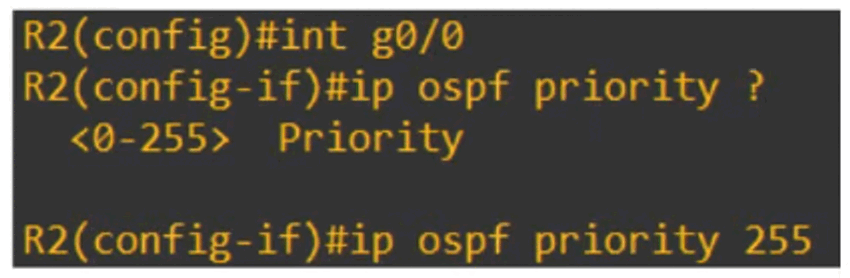
\includegraphics[keepaspectratio,alt={image}]{images/29-ospf-part3/img-004.png}}
\end{figure}

\begin{tipbox}

IF an OSPF PRIORITY is set to ``0'', the ROUTER CANNOT be the DR / BDR
for the SUBNET!

\end{tipbox}

The DR / DBR ELECTION is ``non-preemptive''.

Once the DR / DBR are selected, they will keep their role until OSPF is:

\begin{itemize}
\tightlist
\item
  Reset
\item
  Interface fails
\item
  Is shut down
\item
  etc.
\end{itemize}

\begin{figure}
\centering
\pandocbounded{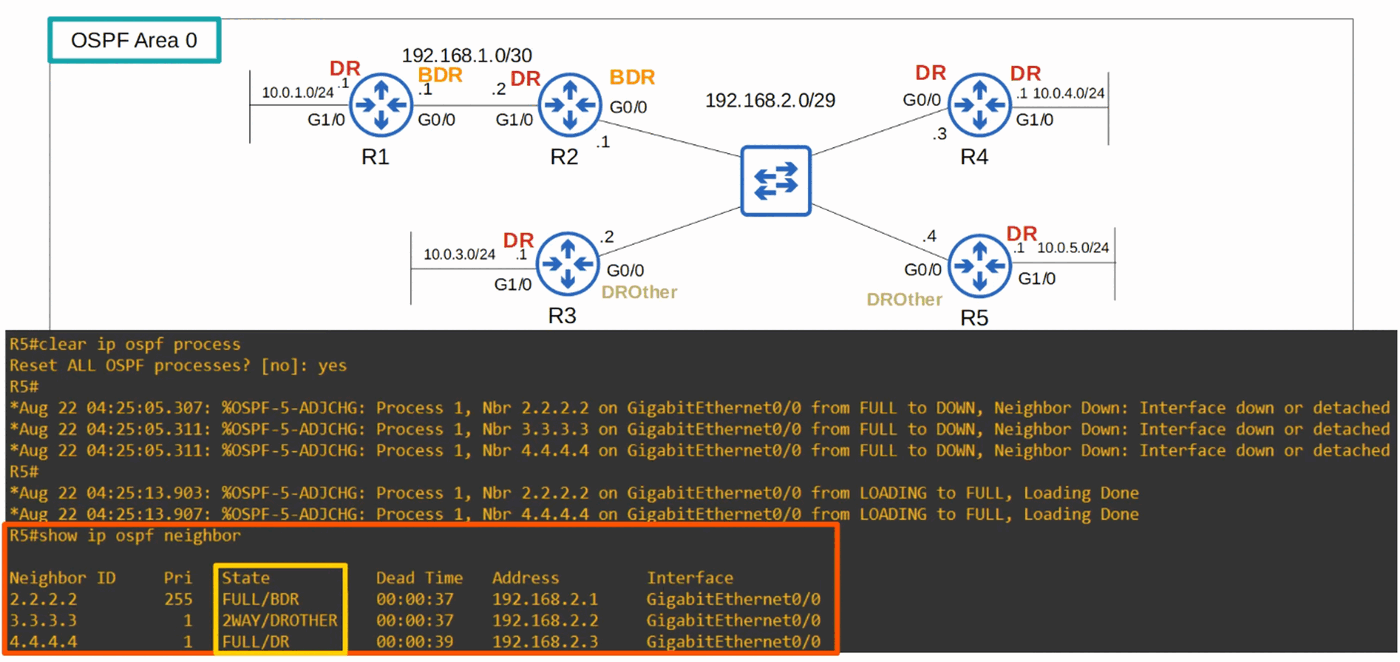
\includegraphics[keepaspectratio,alt={image}]{images/29-ospf-part3/img-005.png}}
\end{figure}

\begin{figure}
\centering
\pandocbounded{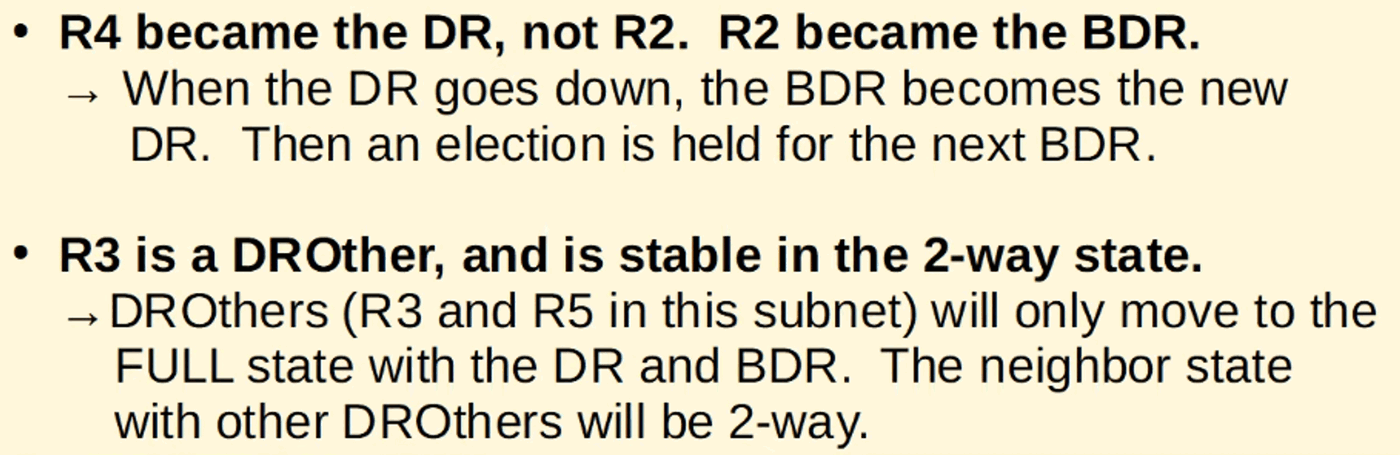
\includegraphics[keepaspectratio,alt={image}]{images/29-ospf-part3/img-006.png}}
\end{figure}

\begin{tipbox}

In the BROADCAST NETWORK TYPE, ROUTERS will only form a FULL OSPF
ADJACENCY with the DR and the BDR of the SEGMENT!

\end{tipbox}

Therefore, ROUTERS only exchange LSAs with the DR and BDR.

DROthers will NOT exchange LSAs with each other.

ALL ROUTERS will still have the same LSDB but THIS reduces the amount of
LSAs flooding the NETWORK

\begin{tipbox}

MESSAGES to the DR / BDR are MULTICAST to 224.0.0.6

\end{tipbox}

The DR and BDR will form a FULL ADJACENCY with ALL ROUTERS in the SUBNET

DROthers will form a FULL ADJACENCY ONLY with the DR / BDR !

\begin{figure}
\centering
\pandocbounded{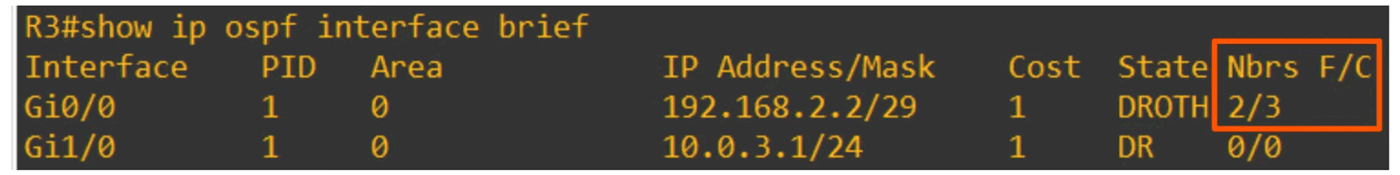
\includegraphics[keepaspectratio,alt={image}]{images/29-ospf-part3/img-007.png}}
\end{figure}

\section{OSPF Point-to-Point Network
Type}\label{ospf-point-to-point-network-type}

\begin{figure}
\centering
\pandocbounded{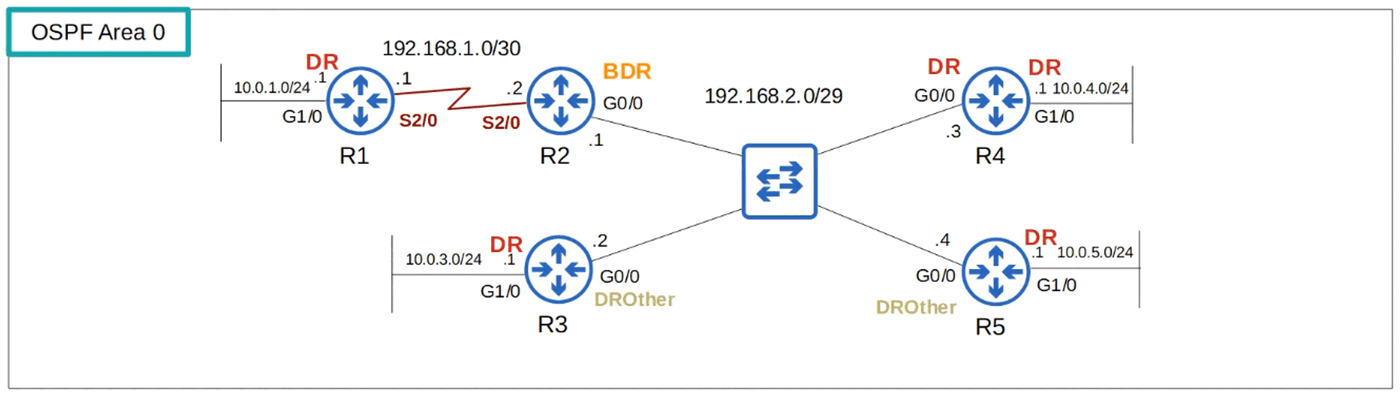
\includegraphics[keepaspectratio,alt={image}]{images/29-ospf-part3/img-008.png}}
\end{figure}

\begin{itemize}
\tightlist
\item
  ENABLED on \textbf{SERIAL} INTERFACES using the \textbf{PPP} and
  \textbf{HDLC} encapsulations, by DEFAULT
\item
  ROUTERS dynamically discover neighbors by SENDING / LISTENING for OSPF
  ``Hello'' messages using the multicast address 224.0.0.5
\item
  A DR and BDR are NOT elected
\item
  These ENCAPSULATIONS are used for ``Point-To-Point'' connections

  \begin{itemize}
  \tightlist
  \item
    Therefore, there is no point in electing a DR and DBR
  \item
    The TWO ROUTERS will form a FULL ADJACENCY with each other
  \end{itemize}
\end{itemize}

(ASIDE)

\section{Serial Interfaces}\label{serial-interfaces}

\begin{figure}
\centering
\pandocbounded{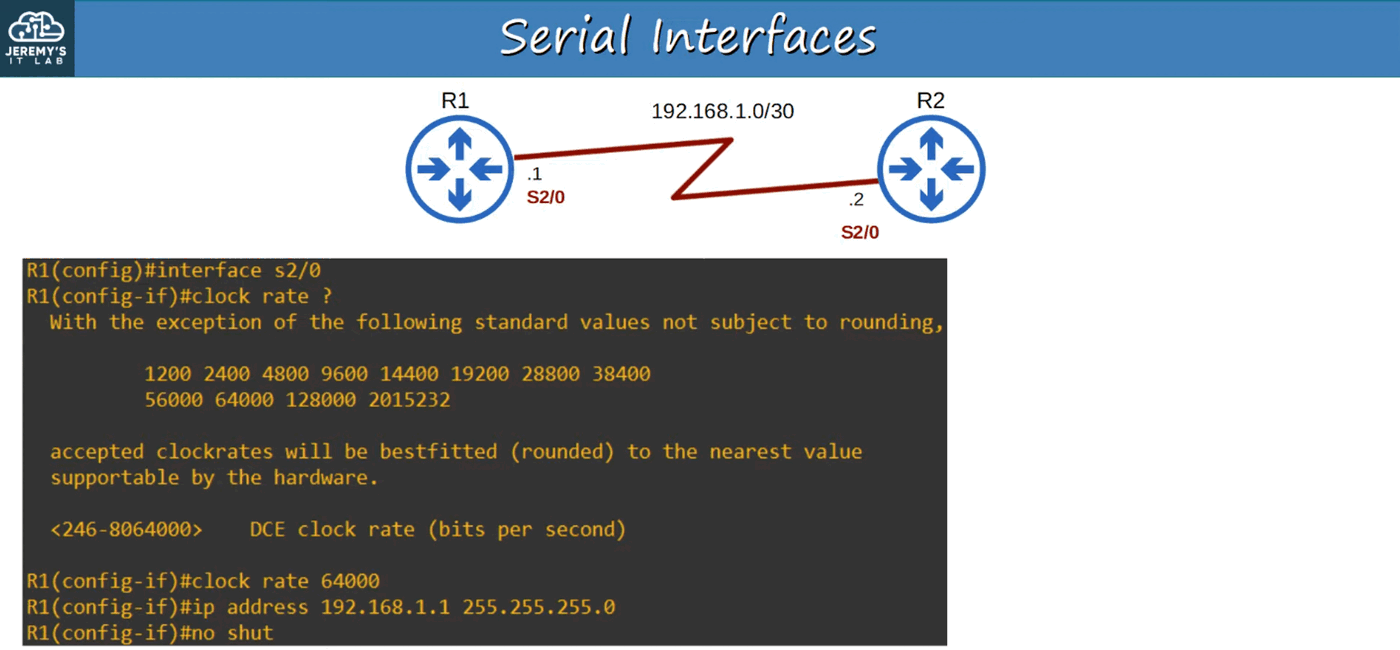
\includegraphics[keepaspectratio,alt={image}]{images/29-ospf-part3/img-009.png}}
\end{figure}

\begin{itemize}
\tightlist
\item
  One side of SERIAL CONNECTION functions as DCE (Data Communications
  Equipment)
\item
  The OTHER side functions as DTE (Data Terminal Equipment)
\item
  ONLY the DCE side needs to specify the \emph{clock rate} (speed) of
  the connection
\end{itemize}

ETHERNET INTERFACES use the ``speed'' command to configure the operating
speed.

SERIAL INTERFACES use the ``clock rate'' command

\begin{figure}
\centering
\pandocbounded{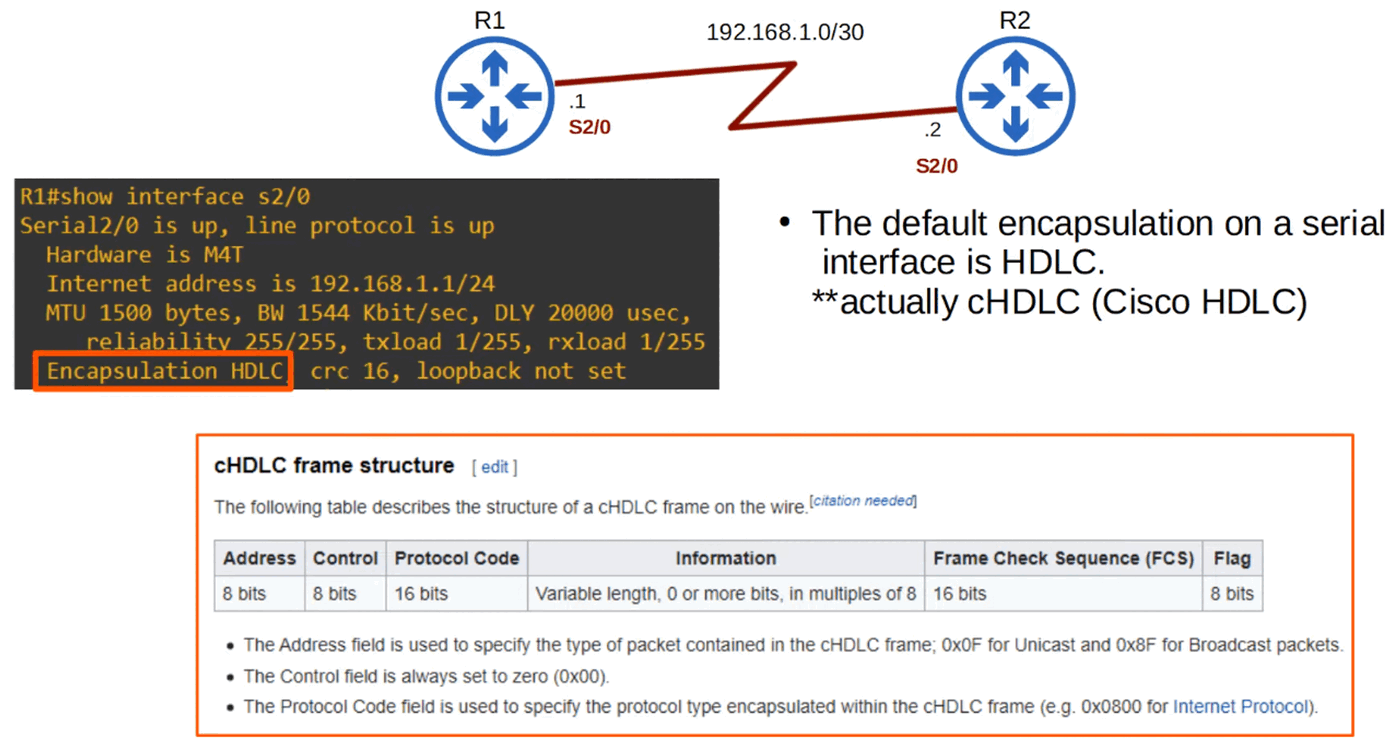
\includegraphics[keepaspectratio,alt={image}]{images/29-ospf-part3/img-010.png}}
\end{figure}

If you change the ENCAPSULATION, it must MATCH on BOTH ENDS or the
INTERFACE will go down.

\begin{figure}
\centering
\pandocbounded{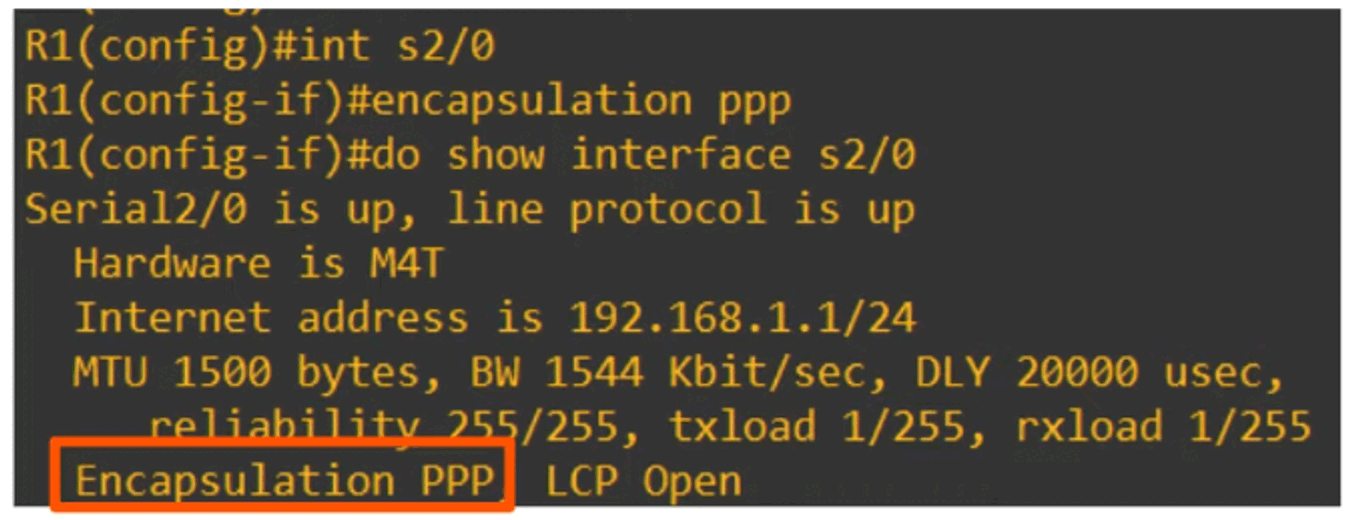
\includegraphics[keepaspectratio,alt={image}]{images/29-ospf-part3/img-011.png}}
\end{figure}

R1 and R2 sharing the SAME Encapsulation Type

\begin{figure}
\centering
\pandocbounded{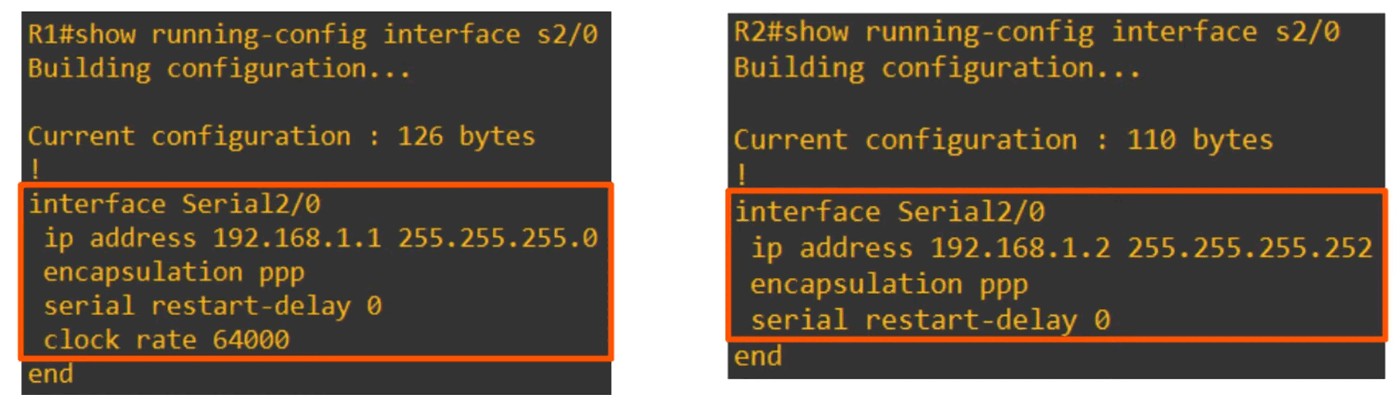
\includegraphics[keepaspectratio,alt={image}]{images/29-ospf-part3/img-012.png}}
\end{figure}

\section{Serial Interfaces Summary}\label{serial-interfaces-summary}

\begin{itemize}
\tightlist
\item
  The DEFAULT encapsulation is HDLC
\item
  You can configure PPP encapsulation with this command:
\end{itemize}

\begin{tipbox}

R1(config-if)\# \textbf{encapsulation ppp}

\end{tipbox}

\begin{itemize}
\tightlist
\item
  One side is DCE, other side is DTE
\item
  Identify which side is DCE / DTE :
\end{itemize}

\begin{tipbox}

R1\# \textbf{show controllers} \emph{interface-id}

\end{tipbox}

\begin{itemize}
\tightlist
\item
  You must configure the CLOCK RATE on the DCE side:
\end{itemize}

\begin{tipbox}

R1(config-if)\# clock rate \emph{bits-per-second}

\end{tipbox}

\begin{figure}
\centering
\pandocbounded{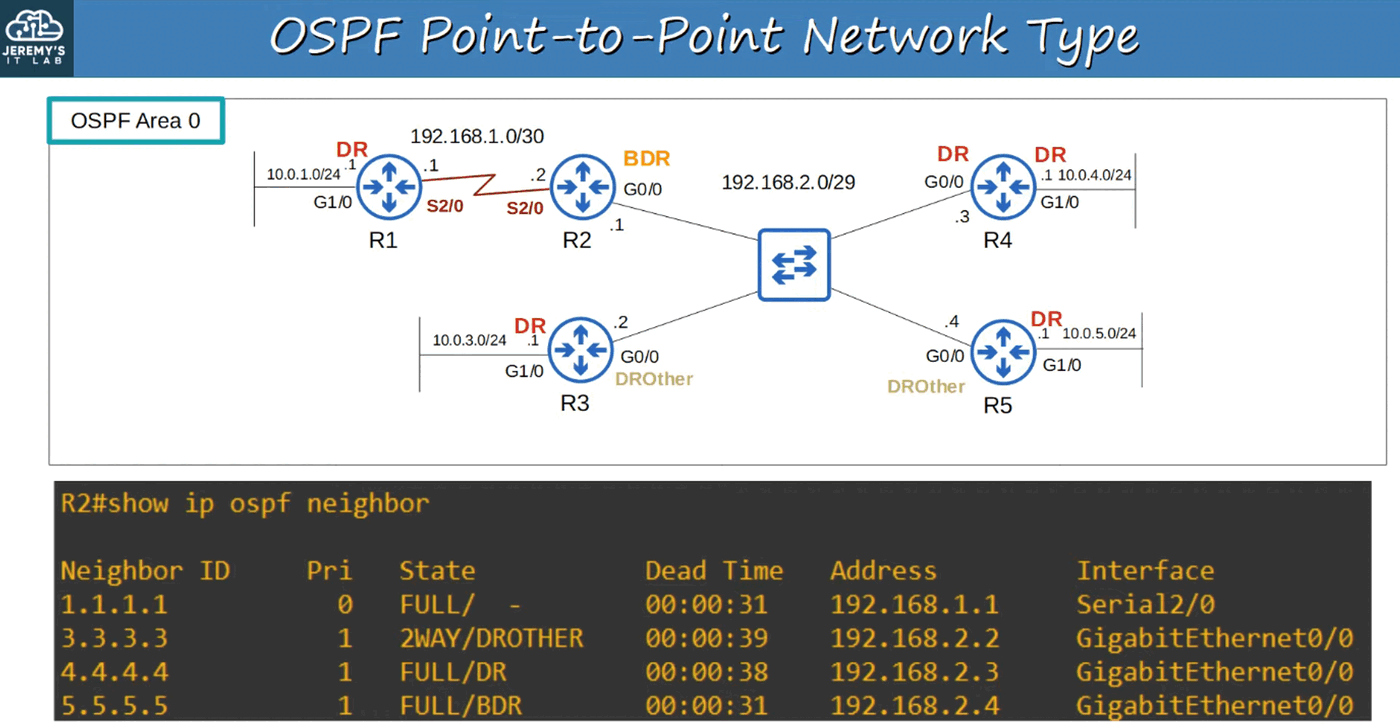
\includegraphics[keepaspectratio,alt={image}]{images/29-ospf-part3/img-013.png}}
\end{figure}

\begin{figure}
\centering
\pandocbounded{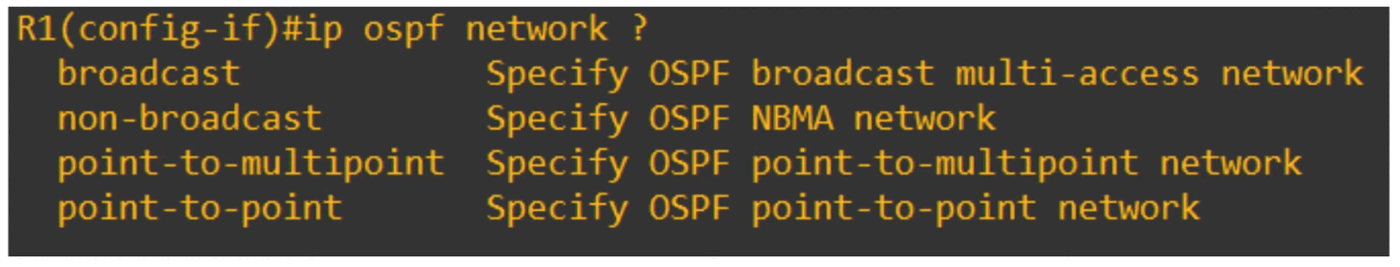
\includegraphics[keepaspectratio,alt={image}]{images/29-ospf-part3/img-014.png}}
\end{figure}

\begin{itemize}
\tightlist
\item
  You can configure the OSPF NETWORK TYPE on an INTERFACE with :
\end{itemize}

\begin{tipbox}

R1(config-if)\# ip ospf network \textless network type\textgreater{}

\end{tipbox}

For example, if TWO ROUTES are directly connected with an ETHERNET link,
there is no need for a DR / DBR. You can configure the POINT-TO-POINT
NETWORK type in this case

NOTE: Not all NETWORK TYPES work on ALL LINK TYPES (for example, a
serial link cannot use the BROADCAST NETWORK type)

\begin{figure}
\centering
\pandocbounded{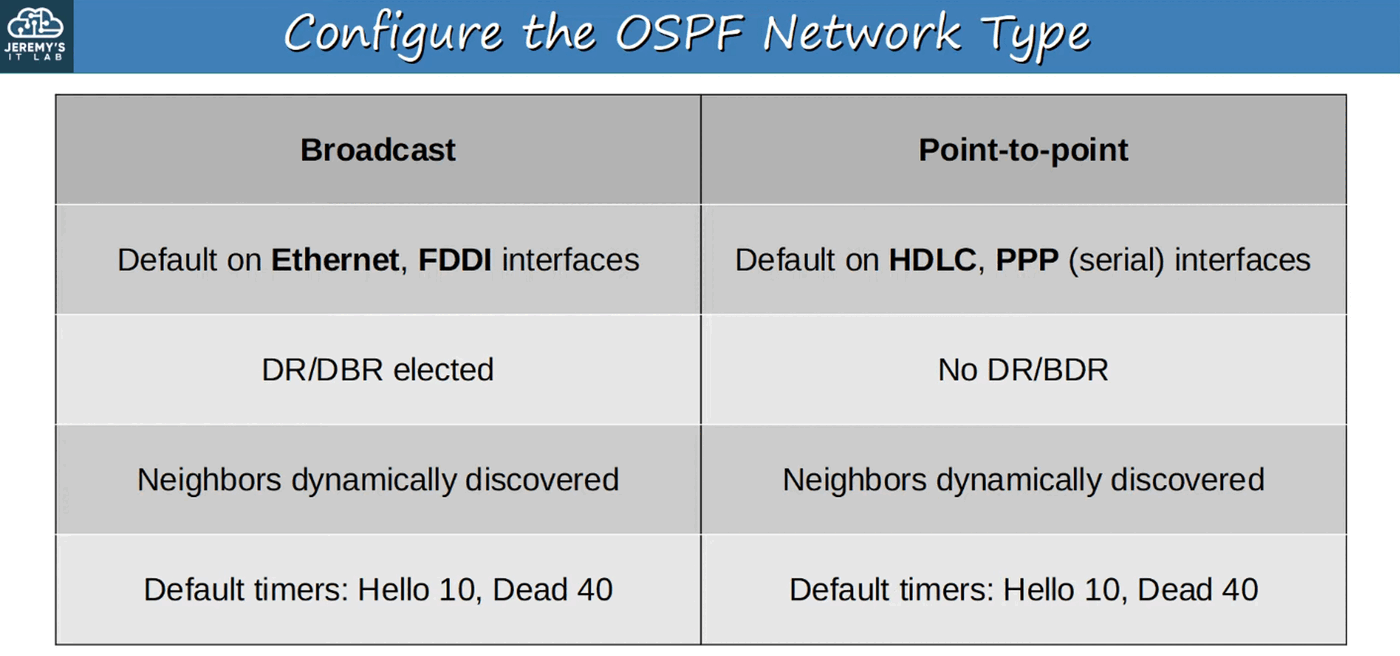
\includegraphics[keepaspectratio,alt={image}]{images/29-ospf-part3/img-015.png}}
\end{figure}

\begin{tipbox}

NON-BROADCAST NETWORK type Default Timers : Hello 30, Dead 120

\end{tipbox}

\section{OSPF Neighbour / Adjacency
Requirements}\label{ospf-neighbour-adjacency-requirements}

\begin{enumerate}
\def\labelenumi{\arabic{enumi})}
\item
  AREA NUMBER MUST MATCH
\item
  INTERFACES must be in the SAME SUBNET
\item
  OSPF PROCESS must not be \textbf{SHUTDOWN}
\end{enumerate}

\begin{figure}
\centering
\pandocbounded{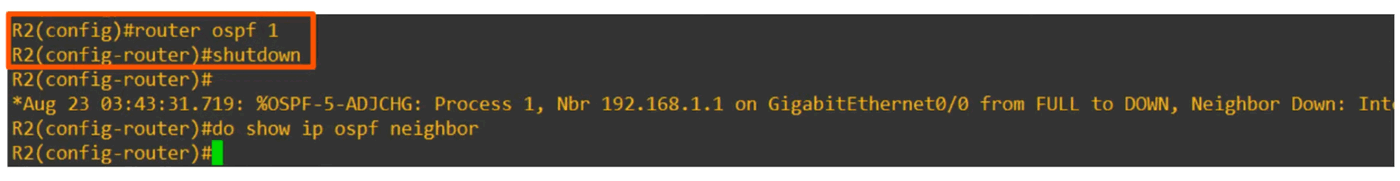
\includegraphics[keepaspectratio,alt={image}]{images/29-ospf-part3/img-016.png}}
\end{figure}

\begin{enumerate}
\def\labelenumi{\arabic{enumi})}
\setcounter{enumi}{3}
\tightlist
\item
  OSPF ROUTER ID must be unique
\end{enumerate}

\begin{figure}
\centering
\pandocbounded{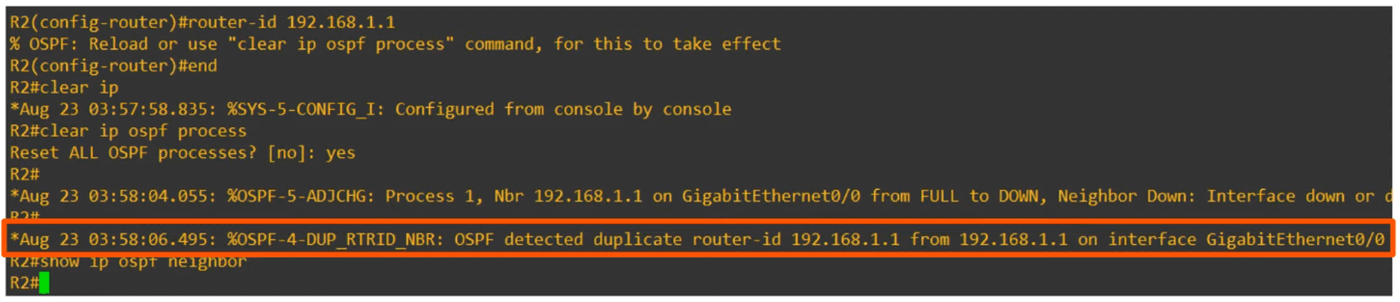
\includegraphics[keepaspectratio,alt={image}]{images/29-ospf-part3/img-017.png}}
\end{figure}

\begin{enumerate}
\def\labelenumi{\arabic{enumi})}
\setcounter{enumi}{4}
\item
  HELLO and DEAD Timers must MATCH
\item
  AUTHENTICATION settings must MATCH
\end{enumerate}

\begin{figure}
\centering
\pandocbounded{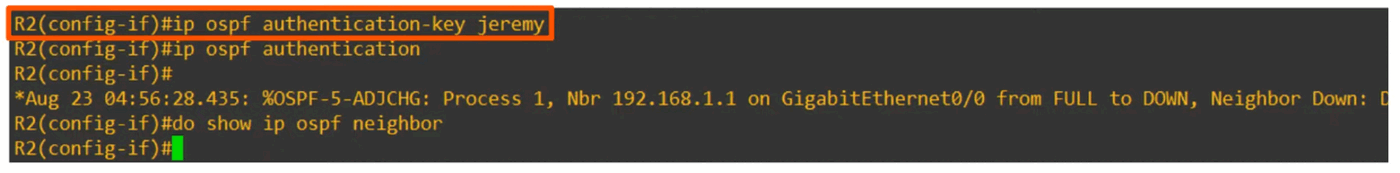
\includegraphics[keepaspectratio,alt={image}]{images/29-ospf-part3/img-018.png}}
\end{figure}

*** SPECIAL REQUIREMENTS ***

\begin{enumerate}
\def\labelenumi{\arabic{enumi})}
\setcounter{enumi}{6}
\tightlist
\item
  IP MTU settings must MATCH
\end{enumerate}

\begin{itemize}
\tightlist
\item
  IP MTU : Maximum size of an IP Packet that can be sent from an
  INTERFACE
\item
  If the settings DO NOT match, can still become OSPF Neighbors but OSPF
  WILL NOT operated properly
\end{itemize}

\begin{enumerate}
\def\labelenumi{\arabic{enumi})}
\setcounter{enumi}{7}
\tightlist
\item
  OSPF NETWORK TYPE must match
\end{enumerate}

\begin{itemize}
\tightlist
\item
  will appear to be working but NEIGHBOR won't appear in ROUTING
  information
\end{itemize}

\section{OSPF LSA Types}\label{ospf-lsa-types}

\begin{itemize}
\tightlist
\item
  The OSPF LSDB is made up of LSAs
\item
  There are 11 types of LSA but there are only 3 you should be aware of
  for the CCNA:

  \begin{itemize}
  \tightlist
  \item
    Type 1 (Router LSA)
  \item
    Type 2 (Network LSA)
  \item
    Type 5 (AS External LSA)
  \end{itemize}
\end{itemize}

TYPE 1 (Router LSA)

\begin{itemize}
\tightlist
\item
  Every OSPF ROUTER generates this type of LSA
\item
  It identifies the ROUTER using it's ROUTER ID
\item
  It also lists NETWORKS attached to the ROUTER's OSPF-Activated
  INTERFACES
\end{itemize}

TYPE 2 (Network LSA)

\begin{itemize}
\tightlist
\item
  Generated by the DR of EACH ``multi-access'' NETWORK (ie: the
  BROADCAST network type)
\item
  Lists the ROUTERS which are attached to the multi-access NETWORK
\end{itemize}

TYPE 5 (AS-External LSA)

\begin{itemize}
\tightlist
\item
  Generated by ASBRs to describe ROUTES to DESTINATIONS outside of the
  AS (OSPF Domain)
\end{itemize}
